% chap3.tex (Chapter 3 of the thesis)

\chapter[INCOMPRESSIBLE NONLINEAR SHALLOW ATMOSPHERE MODEL]{INCOMPRESSIBLE NONLINEAR SHALLOW ATMOSPHERE MODEL}
\label{chap:3}
The goal of this chapter is two fold: Firstly we wish to extend the linearized solutions computed in Chapter~\ref{chap:2} to encompass the fully nonlinear equation set for the dynamical system. This will allow for the investigation of subtleties in the flow field, resulting from nonlinearity, which are not possible to expose using linear theory alone. Secondly, and perhaps more importantly, we aim to conduct an in-depth study of the relationship between the progressive wavespeed and corresponding amplitude. As will be shown, this type of analysis can reveal some interesting results concerning Rossby wave behaviour. It will be demonstrated that solutions of the system are highly dependent on the wavenumber $\kappa$ and the zonal flow angular speed $\omega$.
\section{Problem Specification}
\subsection{Conservation Equations}
The equations of motion to be used in the present chapter are those derived in the previous chapter for conservation of mass and momentum in the rotating shallow atmosphere system. For ease of reference and completeness we restate these equations (\eqref{eq:massincom2non}, \eqref{eq:lamincom2non} and \eqref{eq:phiincom2non}) here for later use. Readers may consult the first few sections of the previous chapter for their derivation. In dimensionless variables we have:
\index{shallow atmosphere equations!non-dimensional incompressible}

{\bfseries mass}
\begin{equation}
\left(u_{\scriptscriptstyle \lambda}-\mathrm{Sr}\,c\cos\phi\right)\frac{\partial \, h}{\partial \, \eta} + u_{\scriptscriptstyle \phi}\cos\phi\frac{\partial \, h}{\partial \, \phi}+h\left[\frac{\partial \, u_{\scriptscriptstyle \lambda}}{\partial \, \eta}+\cos\phi\frac{\partial \, u_{\scriptscriptstyle \phi}}{\partial \, \phi}-u_{\scriptscriptstyle \phi}\sin\phi\right]=0, \label{eq:massincom2nonlin}
\end{equation}
{\bfseries \boldmath$\lambda$ momentum}
\begin{equation}
\left(u_{\scriptscriptstyle \lambda}-\mathrm{Sr}\,c\cos\phi\right)\frac{\partial \, u_{\scriptscriptstyle \lambda}}{\partial \, \eta} + u_{\scriptscriptstyle \phi}\cos\phi\frac{\partial \, u_{\scriptscriptstyle \lambda}}{\partial \, \phi} - \left(\frac{\cos\phi}{\mathrm{Ro}} + u_{\scriptscriptstyle \lambda}\right)u_{\scriptscriptstyle \phi}\sin\phi + \frac{1}{\mathrm{Fr}^2}\frac{\partial \, h}{\partial \, \eta} = 0, \label{eq:lamincom2nonlin}
\end{equation}
{\bfseries \boldmath$\phi$ momentum}
\begin{equation}
\left(u_{\scriptscriptstyle \lambda}-\mathrm{Sr}\,c\cos\phi\right)\frac{\partial \, u_{\scriptscriptstyle \phi}}{\partial \, \eta} + u_{\scriptscriptstyle \phi}\cos\phi\frac{\partial \, u_{\scriptscriptstyle \phi}}{\partial \, \phi} + \left(\frac{\cos\phi}{\mathrm{Ro}} + u_{\scriptscriptstyle \lambda} \right)u_{\scriptscriptstyle \lambda}\sin\phi + \frac{\cos\phi}{\mathrm{Fr}^2}\frac{\partial \, h}{\partial \, \phi} = 0. \label{eq:phiincom2nonlin}
\end{equation}
The analytical solution of the above set of equations is extremely difficult, if not impossible, so we must turn to numerical approximation techniques to find solutions of the system. We will again employ the use of \index{Fourier series}Fourier series but we must now use series with basis functions that span the entire solution range, rather than a restricted sub-domain as in the linearized solution approach.

\subsection{Series Representation} \index{series representation}
In the previous chapter we were able to make use of the concept of a zonal flow and consider small perturbations about it. This approach allowed us to find small linearized corrections to the general flow field. In particular we showed that the two zonal flow parameters $\omega$ and $h_o$ were enough to specify completely any zonal flow configuration. In the present chapter we still wish to use the concept of a zonal flow but we must now incorporate this into our series expansions as a fundamental component of the solution. Additionally, it is no longer possible to use the constant of integration $h_o$ as a zonal flow parameter. This is because $h_o$ effectively controls the free-surface height at the poles and in the nonlinear model we have no way of knowing what this height will be. Instead, the polar height becomes an output of the model and we must use some other technique for controlling the zonal flow state. We will address this issue shortly but first we define the particular forms for each series expansion.

Taking the symmetry and boundary conditions of Section~\ref{subsec:incomplinser} in Chapter~\ref{chap:2} we now generalise the restricted series forms \eqref{eq:Lamseries}, \eqref{eq:Phiseries} and \eqref{eq:Hseries} to encompass a wider range of solution. We can show that the series for the nonlinear problem that meet our conditions are given by:
\begin{align}
\ulam(\eta,\phi) &= \omega\cos\phi+\sum_{m=1}^\infty \sum_{n=1}^\infty P_{m,n}\cos(\kappa m \eta) \cos\bigl((2n-1)\phi\bigr), \label{eq:Lamseriesfull}\\
\uphi(\eta,\phi) &= \sum_{m=1}^\infty \sum_{n=1}^\infty Q_{m,n}\sin(\kappa m \eta) \sin(2n\phi), \label{eq:Phiseriesfull}\\
h(\eta,\phi) &= \sum_{n=0}^\infty H_{0,n}\cos(2 n \phi) \notag \\
&\quad+\sum_{m=1}^\infty \sum_{n=1}^\infty H_{m,n} \cos(\kappa m \eta) (-1)^n \left[ \cos(2n\phi)+\cos\bigl(2(n-1)\phi\bigr) \right], \label{eq:Hseriesfull}
\end{align}
where \eqref{eq:Hseriesfull} uses basis recombination to satisfy boundary conditions at the poles and the series \eqref{eq:Lamseriesfull} for $\ulam$ now contains the primary zonal flow velocity component. Instead of specifying the polar free-surface height we replace $h_o$ with the $\eta$-independent series in \eqref{eq:Hseriesfull} to allow for the polar height to be determined from the output of the model, as discussed previously.

It is interesting to point out the absence of any $\eta$-independent terms in the series \eqref{eq:Lamseriesfull} apart from the primary zonal flow term. One might well assume that to span the solution space with a complete basis set one should use a series for $\ulam$ of the form
\begin{equation*}
\ulam(\eta,\phi) = \omega\cos\phi+\sum_{n=1}^\infty P_{0,n} \cos\bigl((2n-1)\phi\bigr)+\sum_{m=1}^\infty \sum_{n=1}^\infty P_{m,n}\cos(\kappa m \eta) \cos\bigl((2n-1)\phi\bigr)
\end{equation*}
where we can think of the additional $\eta$-independent series term as modifying the base zonal flow in a way that only depends on latitude. The problem with this approach is that the zonal flow is no longer unique.  Any numerical scheme that attempts to solve the equations using this series representation will fail since the zonal flow now becomes an output of the problem and the system has no way of knowing its own base state. In hindsight this conclusion seems rather obvious; however it was not discovered until analysis of the \index{singular value decomposition}singular value decomposition of the Jacobian of the truncated system revealed exactly $N$ machine precision sized singular values in the spectrum corresponding to the coefficients $P_{0,1}$ to $P_{0,N}$. Removal of these terms subsequently removed any associated ill-conditioning in the Jacobian, allowing the solution to be computed.

\subsection{Volume Specification} \index{volume specification}
To be able to make comparison between various solutions we need to fix the total mass of the system. The incompressibility of the problem implies that the density is constant throughout the fluid and hence we may regard conservation of mass as being equivalent to conservation of volume. To calculate the total volume of the fluid we integrate over the region contained between the surface of the sphere and the free-surface so that
\begin{align}
V_{nl}&=\int\limits_0^{2\pi} \int\limits_{-\pi/2}^{\pi/2} \int\limits_{\hat{a}}^{\hat{a}+h(\eta,\phi)} r^2 \cos\phi\,dr d\phi d\eta \notag  \\
&=\frac{4\kappa}{3} \int\limits_0^{\pi/\kappa} \int\limits_0^{\pi/2} \left[ h^3 +3\hat{a}^2h+3\hat{a}h^2  \right]\cos\phi \,d\phi d\eta, \label{eq:volnl}
\end{align}
where $\hat{a}$ is the dimensionless form of the sphere's radius. Note also that we retain the wavenumber parameter \index{$\kappa$, longitudinal wavenumber}$\kappa$ from the previous chapter as a means of controlling the longitudinal wavelength and as a consequence we can restrict our integration to a smaller domain since the free-surface will have \index{symmetry conditions}symmetry about the coordinate line $\eta =\pi/\kappa$.

To use the volume conservation condition effectively we need to decide upon a specific value for the volume, which we will denote \index{$V_z$, zonal flow volume}$V_z$. Once this volume has been established we can construct an equation that reflects volume conservation by equating this volume with the volume obtained from \eqref{eq:volnl}. Thus we have the nonlinear equation for volume conservation given by
\begin{equation}
1-\frac{V_{nl}}{V_z}=0. \label{eq:volcon}
\end{equation}

Equation \eqref{eq:volcon} effectively replaces the specification of $h_o$ to define an unique zonal flow structure. In the linearized problem an equivalent equation to \eqref{eq:volcon} was not required since, for a fixed value of $\omega$, the volume remained constant because the wavespeed did not vary with changes in the wave amplitude. In the nonlinear problem it is possible to have many different flow configurations for the same value of $\omega$ since the wavespeed now depends on the wave amplitude and thus the resulting volume will change as the Rossby wave amplitude changes. By using \eqref{eq:volcon} we force the volume to remain constant for all computed solutions. If the amplitude is changing and the volume is constant it implies that the mean height of the fluid must either increase or decrease. The mean height of the fluid is controlled via the polar free-surface height $h_o$. It is now apparent that we have in fact parametrised the \index{polar height parametrisation}polar height $h_o$ in terms of the conservation condition expressed in \eqref{eq:volcon}, and this becomes the extra condition to close the problem.

\section{Numerical Solution Method}
\subsection{Collocation}
Equations \eqref{eq:massincom2nonlin}, \eqref{eq:lamincom2nonlin}, \eqref{eq:phiincom2nonlin} and \eqref{eq:volcon} constitute a complete system for which the solution gives nonlinear Rossby waves. The solution process consists of finding the coefficients $H_{m,n}$, $P_{m,n}$, $Q_{m,n}$ and wavespeed $c$ that make the series \eqref{eq:Lamseriesfull}, \eqref{eq:Phiseriesfull} and \eqref{eq:Hseriesfull} a solution of the system. Various different techniques for doing this are possible. The method chosen here is the pseudospectral technique of collocation\index{collocation method} in which we require the residuals, obtained by substituting the series into the governing equations, to be zero at every point on a mesh constructed from a finite number of points in the flow field. This technique is in contrast to the spectral \index{Galerkin method}Galerkin method of the previous chapter in which we required the residuals to be orthogonal to the basis expansion functions over the entire domain. While we can use the same basis functions for both the collocation and the Galerkin method, in the collocation method we no longer have the residual orthogonality property of spectral methods in general.

There are both advantages and disadvantages to using the \index{collocation method!advantages}collocation method over other techniques such as the Galerkin method or \index{finite-difference scheme}finite-difference schemes. Durran\cite[pages 191--195]{Duran:NMW} presents a detailed exposition of these key differences. In summary, the main advantage of collocation over a finite-difference scheme is that the collocation method will be more accurate provided the solution is smooth. This is a direct result of using infinitely differentiable basis functions which allow for the calculation of exact function derivatives at each point in the flow domain. The main advantage of collocation over the Galerkin method is that the collocation method is computationally less intensive because costly integrals need not be evaluated at each step. In addition, since the grid points are fixed for a particular mesh, we can \index{basis function!caching}cache the basis functions and their derivatives at all necessary points and use these stored values to speed up the solution process by eliminating costly function calls in the program. This technique will be explained later in the chapter.

The book by Boyd\cite{Boyd:CFSM} provides an extensive analysis of spectral and \index{pseudospectral method}pseudospectral methods, from which we summarise the basic process of the \index{collocation method!algorithm}collocation method as follows. Suppose we have some functional operator given by
\begin{equation}
F[y(x)]=0, \label{eq:Fofy}
\end{equation}
for independent variable $x$ and dependent variable $y$. To solve this problem numerically we approximate $y(x)$ with a truncated series expansion of orthogonal basis functions, $\psi_n(x)$, so that
\begin{equation}
y(x)\approx y_N(x)= \sum_{n=0}^N a_n \psi_n(x). \label{eq:yapprox}
\end{equation}
Substituting \eqref{eq:yapprox} into \eqref{eq:Fofy} yields the equation
\begin{equation}
E[a_0,a_1,\ldots,a_N,x]=F[y_N(x)]=0. \label{eq:Eofx}
\end{equation}
We now choose $N+1$ points, $x_0,\ldots,x_N$, from the function domain and evaluate \eqref{eq:Eofx} at each of these discrete values to give
\begin{equation}
\bol{E(\bol{a})}=\bol{0}, \label{eq:Evec}
\end{equation}
where \bol{a} is the vector of unknown coefficients. In general \eqref{eq:Evec} will not be satisfied for arbitrary \bol{a} and it now becomes the task to find the coefficients $a_0,a_1,\ldots,a_N$ that will simultaneously satisfy each individual component equation in \eqref{eq:Evec}.

The above algorithm outlines the essential elements of any collocation method. That is; find series coefficients that satisfy the residual equations exactly at a discrete number of points taken from the solution domain. A variety of methods can be employed to find the minimising set of coefficients; however it must be emphasized that this step is distinct from the general collocation method as a whole. In addition, the particular choice of grid points $x_i$ is also an important stage in the solution process since certain choices of points are optimal in the sense of satisfying the equations at non-grid points. For our purposes the choice is easy since one can show that for Fourier basis functions the \index{collocation mesh!optimal choice}optimal choice is an evenly spaced mesh of grid points \cite{Boyd:CFSM}. We now address the sub-task of finding the optimal set of coefficients $a_n$.

\subsection{Newton--Raphson Technique} \label{sec:NewRap} \index{Newton--Raphson method}
In general, the task of finding the vector of unknown coefficients \bol{a} that satisfies equation \eqref{eq:Evec} is labelled a multi-dimensional \index{root finding!multi-dimensional}root finding problem. Problems of this type are notoriously difficult for a number of reasons, the main one being that zeros of one residual component generally have nothing in common with zeros of another distinct residual component, as described in Press et~al.\cite[pages 383--386]{Press:NRC}. However, it is possible to solve problems of this type with careful analysis and planning. One such method for accomplishing this task is an iterative technique called the Newton--Raphson algorithm.

We present here an overview of the Newton--Raphson \index{Newton--Raphson method!algorithm}algorithm as detailed in \cite[pages 383--386]{Press:NRC}. Suppose we start with some initial guess for the vector of unknown coefficients, defined to be $\bol{a}^{(k)}$ where the superscript denotes the current iterative step. Each individual residual component in \eqref{eq:Evec} can be expanded locally in a Taylor series about the multi-dimensional point $\bol{a}^{(k)}$, leading to the vector equation
\begin{equation}
\bol{E}(\bol{a}^{(k)}+\bol{\delta a}^{(k)})=\bol{E}(\bol{a}^{(k)})+\bol{J}^{(k)}\cdot\bol{\delta a}^{(k)}+O((\bol{\delta a}^{(k)})^2), \label{eq:Taylorapprox}
\end{equation}
where $\bol{J}^{(k)}$ is the \index{Jacobian matrix}Jacobian matrix of partial derivatives and is defined by
\begin{equation}
J^{(k)}_{ij} =\left. \frac{\partial E_i}{\partial a_j} \right|_{\bol{a}^{(k)}}.
\end{equation}
The goal of the root finding process is to make $\bol{E}(\bol{a}^{(k)}+\bol{\delta a}^{(k)})=\bol{0}$; thus equation \eqref{eq:Taylorapprox} provides a recipe for achieving this goal, since as a first approximation we can neglect the higher order terms and set $\bol{E}(\bol{a}^{(k)}+\bol{\delta a}^{(k)})=\bol{0}$, enabling us to solve for the correction step $\bol{\delta a}^{(k)}$ that brings vector $\bol{a}^{(k)}$ closer to satisfying \eqref{eq:Evec}. The resulting linear system for the step direction is given by
\begin{equation}
\bol{J}^{(k)}\cdot\bol{\delta a}^{(k)} = -\bol{E}(\bol{a}^{(k)}),
\end{equation}
which can be solved for the vector $\bol{\delta a}^{(k)}$ using standard linear algebra techniques. Once we have found the updating step, we update the solution to give the new vector
\begin{equation}
\bol{a}^{(k+1)}=\bol{a}^{(k)}+ \bol{\delta a}^{(k)},
\end{equation}
which should be a better approximation to a root of \eqref{eq:Evec}. The above process is then repeated, starting from the new point $\bol{a}^{(k+1)}$, until convergence is achieved.

While this algorithm is useful it is by no means robust in the sense that it will always find a solution if one is known to exist. Specifically, the \index{Newton--Raphson method!shortcomings}Newton--Raphson method is known to converge to a root only if the starting guess is sufficiently close to the root. Thus root finding using this technique requires both care and insight into the expected nature of the solution, as described by Acton~\cite{Acton:NMW}.

One may improve the overall efficiency of the \index{Newton--Raphson method!damped}Newton--Raphson method by implementing a damping mechanism that tests if the calculated solution update at each stage of the algorithm actually does reduce each of the individual residual equations. Since the update vector $\bol{\delta a}^{(k)}$ will always be a descent direction, see~\cite{Press:NRC}, we can test the value of the residual at the new calculated point $\bol{a}^{(k+1)}$ and if $||\bol{E}(\bol{a}^{(k+1)})|| > ||\bol{E}(\bol{a}^{(k)})||$, for some appropriate norm, we reduce the magnitude of the step size by replacing $\bol{\delta a}^{(k)}$ with $\bol{\delta a}^{(k)}/2$ and retesting until we find a step magnitude that does reduce the residual. This technique is essentially the Newton-Raphson method with quasi line searches at the end of each iteration step.

The complete damped Newton--Raphson algorithm is represented in Table~\ref{tab:NewRap}, where $\epsilon_1$ and $\epsilon_2$ are user-prescribed terminating error tolerances. In practice, one would normally use an $L^1$ or $L^2$ norm to represent the total residual error; in this study, the $L^1$ norm is employed. Additionally, step 3 of the algorithm must be monitored closely to check for spurious convergence since halving the step size multiple times will eventually satisfy the second terminating condition expressed in step 5. The simplest possible method to prevent this non-genuine convergence is to have an upper limit on the number of halvings allowed at each iterative level in the algorithm. If this limit is reached the algorithm is deemed to have failed for the specific initial guess in step 1, implying that either a root does not not exist nearby or a new initial guess is required.\index{Newton--Raphson method!algorithmic flow chart}
\begin{table}[htbp]
	\centering
	{\bfseries Damped Newton--Raphson Algorithmic Flow Chart}
	\begin{enumerate}
	\item Define an initial guess, $\bol{a}^{(k)}$.
	\item Solve the linear system, $\bol{J}^{(k)}\cdot\bol{\delta a}^{(k)} = -\bol{E}(\bol{a}^{(k)})$, for $\bol{\delta a}^{(k)}$.
	\item While $||\bol{E}(\bol{a}^{(k)}+\bol{\delta a}^{(k)})|| > ||\bol{E}(\bol{a}^{(k)})||$, do $\bol{\delta a}^{(k)}=\bol{\delta a}^{(k)}/2$
	\item Update the solution, $\bol{a}^{(k+1)}=\bol{a}^{(k)}+ \bol{\delta a}^{(k)}$
	\item If $||\bol{E}(\bol{a}^{(k+1)})|| \le \epsilon_1$ or $||\bol{\delta a}^{(k)}|| \le \epsilon_2$, EXIT
	\item Increment $k$ by 1 and repeat from step~2.
	\end{enumerate}
	\caption{Damped Newton-Raphson algorithm.}
	\label{tab:NewRap}
\end{table}

\section{Code Highlights}
In this section we present a brief overview of the key computer code components used to assemble and solve the nonlinear problem, as well as some specific details for particular techniques that were utilised.
\subsection{Programming Language and Computational Environment}
\label{subsec:compinfo}
C++ was selected as the base programming language. In addition, various algorithms, with appropriate modifications, from ``Numerical Recipes in C++'' by Press~et~al.\cite{Press:NRC} were employed for common tasks, such as the solution of a linear system. The feature rich abilities of the C++ programming language were exploited where possible with much use being made of operator overloading to simplify and improve the readability of code. The Microsoft Visual C++ 6.0 and GNU C++ compilers were used for compilation on Microsoft Windows XP(tm) and Red Hat Linux 9.0(tm) respectively.

The majority of computations were performed on two separate computers, the first being an AMD \index{computer specifications}Athlon(tm) XP 1800+ processor clocked at 1.54~GHz with 512~MB of physical memory clocked at 266~MHz, the second being an Athlon(tm) XP 2800+ processor clocked at 2.08~GHz with 1~GB of dual channel physical memory clocked at 333~MHz. Additionally, some computations were performed on an SGI Origin 3400 high performance computer (24 R14000 (500 MHz) CPUS, 24 GB main memory) using OpenMP, a programming interface for writing high performance parallel computations. Access to the super computer was generously provided by the Tasmanian Partnership for Advanced Computing (TPAC).

\subsection{Truncation} To accomplish the task of numerically solving for the coefficients $H_{m,n}$, $P_{m,n}$, $Q_{m,n}$ and wavespeed $c$, we \index{Fourier series!truncation}truncate the infinite series \eqref{eq:Lamseriesfull}--\eqref{eq:Hseriesfull} with longitudinal truncation $M$ and latitudinal truncation $N$ to give
\begin{align}
\ulam(\eta,\phi) &= \omega\cos\phi+\sum_{m=1}^M \sum_{n=1}^N P_{m,n}\cos(\kappa m \eta) \cos\bigl((2n-1)\phi\bigr), \label{eq:Lamseriestrun}\\
\uphi(\eta,\phi) &= \sum_{m=1}^M \sum_{n=1}^N Q_{m,n}\sin(\kappa m \eta) \sin(2n\phi), \label{eq:Phiseriestrun}\\
h(\eta,\phi) &= \sum_{n=0}^N H_{0,n}\cos(2 n \phi) \notag \\
&\quad+\sum_{m=1}^{M-1} \sum_{n=1}^N H_{m,n} \cos(\kappa m \eta) (-1)^n \left[ \cos(2n\phi)+\cos\bigl(2(n-1)\phi\bigr) \right]. \label{eq:Hseriestrun}
\end{align}
Series \eqref{eq:Lamseriestrun}--\eqref{eq:Hseriestrun}, along with the unknown wavespeed $c$, contain a total of $3MN+2$ unknown coefficients, so in order to close the system numerically we will need the same number of \index{residual equation}residual equations to use in the collocation method. 

We have already noted that the problem is governed by three dynamical equations, \eqref{eq:massincom2nonlin}--\eqref{eq:phiincom2nonlin}, and a volume specification equation, \eqref{eq:volcon}. Since the volume specification equation contains an integral it is not possible to evaluate this at individual points in the domain. Rather, it represents the contribution from every point in the domain. Consequently we can just evaluate this equation once for a given coefficient set and append the result to our residual vector obtained from collocating at discrete points in the domain. This reduces the required number of collocation points to $3MN+1$.

\subsection{Forcing the Solution}
%\index{forcing}We want to be able to control the solution to a certain degree by stipulating either the wave amplitude, denoted $\mathcal{A}$, or the wavespeed, $c$, so that we may investigate the nonlinear dependence of the wavespeed on amplitude. In the linearized theory this dependence was not possible to expose because we were only considering small amplitude waves. In the nonlinear theory it is expected that the wavespeed will be a function of amplitude so that $c\equiv c(\mathcal{A})$. This behaviour has been demonstrated in a variety of situations, the most famous being Stokes'\cite{Stokes:TOW} classic paper on finite amplitude gravity waves which has spawned a plethora of additional papers (see the review article by Schwartz \& Fenton \cite{Schwartz:SNW}). 

\index{forcing}It is necessary to be able to control the solution by stipulating either the wave amplitude, denoted $\mathcal{A}$, or the wavespeed, $c$, so that we may investigate the nonlinear dependence of the wavespeed on amplitude. In the linearized theory this dependence was not possible to expose because we only considered small amplitude waves. In the nonlinear theory the wavespeed will be a function of amplitude so that $c\equiv c(\mathcal{A})$. This behaviour has been demonstrated in a variety of situations, the most famous being Stokes'\cite{Stokes:TOW} classic paper on finite amplitude gravity waves which has spawned a plethora of additional papers (see the review article by Schwartz \& Fenton \cite{Schwartz:SNW}). 

To force either the \index{forcing!wavespeed}wavespeed or \index{forcing!amplitude}amplitude we must hold either of the two constant throughout each root finding process. It is most helpful to hold the amplitude constant and let the wavespeed be an output of the problem. To this end we need a way of specifying the wave amplitude. This can be achieved by noting that we can parameterise $\mathcal{A}$ in terms of one of our unknown coefficients. For example, we can hold $H_{1,1}$ fixed in the series for $h(\eta,\phi)$, thus removing one of the unknowns from the problem. With this method we have no way of knowing exactly what the relationship between $\mathcal{A}$ and $H_{1,1}$ is, but it suffices to know that there {\em is} a relationship, through which we can force $\mathcal{A}$ by specifying individual values for $H_{1,1}$.

By specifying either one of the coefficients or the wavespeed we again reduce by one the total number of unknowns in the problem so that we must now construct a total of $3MN$ residual equations. Since we have 3 separate dynamical equations that govern the system we need a total of $MN$ collocation mesh points. We choose $M$ points from the $\eta$ domain and $N$ points from the $\phi$ domain, to be discussed in the next section.

\subsection{Collocation Points}
For each \index{collocation mesh}orthogonal set of basis functions, there exists an optimal set of points chosen, from the function domain, which will yield an optimal collocation method. In general one can show that the optimal set of grid points consists of the abscissas of a Gaussian quadrature associated with the specific basis set \cite[page 88]{Boyd:CFSM}. For the trigonometric basis functions of a Fourier series, these points are evenly spaced throughout the entire periodic function domain and thus are easily calculated for any given truncation level.

For the collocation points in $\phi$ we restrict ourselves to the Northern hemisphere since our solution has specific symmetry relative to the equator. In addition we choose strictly internal points from the domain since we have imposed boundary conditions at both $\phi=0$ and $\phi=\pm \pi/2$ through the specific choice of our basis functions. Defining 
\begin{equation}
\Delta \phi = \frac{\pi}{2(N+1)} \label{eq:delphi}
\end{equation}
to be the inter-grid point distance in the $\phi$ direction, the $N$ equally-spaced $\phi$-grid points are
\begin{equation}
\phi_i = i \Delta \phi, \quad \text{for } i=1,2,\ldots,N. \label{phigrid}
\end{equation}

The collocation points in $\eta$ can be obtained in a similar manner; however, since we have stipulated a dependence on the wavenumber $\kappa$, we need to consider the effect this has on the linear independence of the individual residual equations. Specifically, if parity exists in the basis functions, and this \index{parity}parity is reflected directly in the residual equations, then the collocation points must be modified to avoid \index{residual equation!redundancy}redundancy in the residual vector \cite[pages 159--171]{Boyd:CFSM}. By incorporating the wavenumber $\kappa$ into our series expansions we effectively force $\kappa$ complete wavelengths around any given \index{latitude circle}latitude circle. In addition each individual wavelength will have symmetry about its midpoint so that, for the first wavelength\footnote{In the expression for $\eta$ the $-ct$ term merely translates any initial wave configuration. We can therefore generalise by letting $t=0$ so that effectively we have $\eta=\lambda$.}, the symmetry line is $\eta = \pi / \kappa$. Consequently we must only choose collocation points from $\eta \in [0,\pi/\kappa)$ to avoid linearly dependent rows in the residual vector and resulting \index{Jacobian matrix!linear dependence}Jacobian matrix. Defining 
\begin{equation}
\Delta \eta = \frac{\pi}{M\kappa} \label{eq:deleta}
\end{equation}
to be the inter-grid point distance in the $\eta$ direction, the $M$ equally spaced $\eta$-grid points are
\begin{equation}
\eta_j = (j-1) \Delta \eta, \quad \text{for } j=1,2,\ldots,M. \label{etagrid}
\end{equation}

The set of points taken from all possible $(\eta_j,\phi_i)$ pairs constitutes what is known as the \index{collocation mesh!definition}collocation mesh. It is at precisely these points, and only these points, that we will zero the individual residual equations by finding the optimising wavespeed and associated set of coefficients. 

\subsection{Caching the Basis Functions}\index{basis function!caching}
Unlike the spectral Galerkin method in which the residual values are considered at every point in the function domain, the pseudospectral collocation method only ever involves a finite number of points from the domain. We can use this to our advantage because generally the most computationally intensive part of any computer program is the evaluation of function calls. Since we know all the points at which we will need to evaluate our basis functions for given truncation levels, we can evaluate these just once and store the results in computer memory for later reference. The equations governing the dynamics contain not only the field variables but their derivatives with respect to $\eta$ and $\phi$ as well, so we can also store this information in computer memory.

To illustrate this concept, \index{basis function!caching example}consider the general basis function $\cos(\kappa m \eta)$ which appears in the $\ulam$ and $h$ series, \eqref{eq:Lamseriestrun} and \eqref{eq:Hseriestrun} , as well as in the $\eta$ derivative of the $\uphi$ series \eqref{eq:Phiseriestrun}. For a given truncation level $M$ the collocation points in $\eta$ are defined uniquely by \eqref{etagrid}. We also know that the index $m$ can take a value ranging from 1 to $M$. We can thus evaluate the general basis function for all possible $m$ and $\eta$ values and store this information in a matrix as
\begin{equation}
\text{C}_{\eta}=\begin{pmatrix} \cos(\kappa \eta_1) & \cdots & \cos(\kappa \eta_M)\\
 \cos(2\kappa \eta_1) & \cdots & \cos(\kappa \eta_M)\\
\vdots &  & \vdots \\
\cos(M \kappa \eta_1) & \cdots & \cos(M \kappa \eta_M) \end{pmatrix}.
\end{equation}

Similar matrices can be constructed and stored in computer memory for all the other general basis functions contained in the series expansions, allowing for rapid array access. 

\subsection{Calculation of the Jacobian Matrix} \index{Jacobian matrix!calculation of}
The root finding process outlined in Section~\ref{sec:NewRap} requires the computation of the Jacobian matrix of the residual vector at each iterative step. There are two main methods usually employed to calculate the Jacobian matrix. The first method involves the use of finite difference approximations to the derivatives of each residual component relative to each member of the vector composed of the unknown coefficients and wavespeed. The second method employs the analytical evaluation of the Jacobian terms prior to the computation stage, resulting in a simple evaluation for each element of the Jacobian. The second method is to be prefered to the first when the Jacobian elements are easily calculated because the resulting evaluations will be accurate to machine precision. In this study the analytical method is employed since the Jacobian elements are, in general, easily determined.

As an example we consider the evaluation of the derivative of the mass equation, \eqref{eq:massincom2nonlin}, with respect to each of our unknown coefficient elements. For the sake of brevity we represent the mass equation at a particular collocation point as $f_1(\bol{a})=0$. Let $a_i$ be a general element of the vector of unknowns \bol{a} and define the function $\psi$ to be a generic placeholder for each of the dependent field variables \ulam, \uphi, $h$ and the wavespeed $c$. We can represent the derivative of $f_1$ with respect to each element of \bol{a} as
\begin{equation}
\frac{\partial f_1}{\partial a_i} = \frac{\partial f_1}{\partial \psi} \frac{\partial \psi}{\partial a_i} + \frac{\partial f_1}{\partial \left(\frac{\partial \psi}{\partial \eta} \right)} \frac{\partial \left(\frac{\partial \psi}{\partial \eta} \right)}{\partial a_i}+ \frac{\partial f_1}{\partial \left(\frac{\partial \psi}{\partial \phi} \right)} \frac{\partial \left(\frac{\partial \psi}{\partial \phi} \right)}{\partial a_i}.
\end{equation}
Using this procedure we can show that the individual Jacobian components for the mass equation are
\begin{align}
\frac{\partial f_1}{\partial P_{i,j}}&=\frac{\partial h}{\partial \eta}\frac{\partial \ulam}{\partial P_{i,j}}+h \frac{\partial \left(\frac{\partial \ulam}{\partial \eta} \right)}{\partial P_{i,j}}, \\
\frac{\partial f_1}{\partial Q_{i,j}}&=\left(\cos\phi\frac{\partial h}{\partial \phi}-h\sin\phi \right)\frac{\partial \uphi}{\partial Q_{i,j}}+h \cos\phi \frac{\partial \left(\frac{\partial \uphi}{\partial \phi} \right)}{\partial Q_{i,j}}, \\
\frac{\partial f_1}{\partial H_{i,j}}&=\left(\frac{\partial \ulam}{\partial \eta}+\cos\phi\frac{\partial \uphi}{\partial \phi}-\uphi \sin\phi \right)\frac{\partial h}{\partial H_{i,j}} \notag \\
&\quad+(\ulam-\mathrm{Sr}c\cos\phi)\frac{\partial \left(\frac{\partial h}{\partial \eta} \right)}{\partial H_{i,j}} +\uphi \cos\phi \frac{\partial \left(\frac{\partial h}{\partial \phi} \right)}{\partial H_{i,j}} \\
\frac{\partial f_1}{\partial c}&=-\mathrm{Sr}\cos\phi \frac{\partial h}{\partial \eta}.
\end{align}
Similar expressions can be obtained for the $\lambda$ and $\phi$ momentum equations. The derivatives of the field variables with respect to each coefficient are readily calculated from the individual series expansions. For example,
\begin{equation}
\frac{\partial \ulam}{\partial P_{i,j}} = \cos(\kappa i \eta)\cos\bigl((2j-1)\phi\bigr).
\end{equation} 
Using this method we populate $3MN$ rows of the Jacobian matrix corresponding to all $3MN$ collocation grid points. 

In addition we must also calculate the Jacobian elements corresponding to the volume specification equation \eqref{eq:volcon}. Since this equation is independent of $\ulam$, $\uphi$ and $c$, the only contribution to the Jacobian will come from derivatives with respect to the free-surface coefficients. Letting the volume specification equation be represented by $f_4(\bol{a})=0$, we have
\begin{equation}
\frac{\partial f_4}{\partial H_{i,j}} = -\frac{4\kappa}{V_z} \int\limits_0^{\pi/\kappa} \int\limits_0^{\pi/2} \left[ h^2 +\hat{a}^2+2\hat{a}h  \right]\frac{\partial h}{\partial H_{i,j}}\cos\phi \,d\phi\, d\eta \label{eq:Voljac}
\end{equation}
where
\begin{equation}
\frac{\partial h}{\partial H_{i,j}}=\begin{cases} \cos(2j\phi)& \text{if} \begin{cases}\begin{array}{l} i=0, \\ j=0,\ldots,N,\end{array}\end{cases} \\[5mm]
\cos(\kappa i \eta)(-1)^j\left[\cos(2j\phi)+\cos \bigl(2(j-1)\phi \bigr) \right]& \text{if} \begin{cases} \begin{array}{l} i=1,\ldots,M-1, \\ j=1,\ldots,N. \end{array}\end{cases} 
\end{cases} \label{eq:dhdH}
\end{equation}
Equation \eqref{eq:Voljac} can be simplified further by analytically evaluating components of the integral that allow manipulation. Appendix~\ref{App:1} contains the specific details.

\subsection{Adaptive Integration Method}
The integrals appearing in \eqref{eq:volnl} and \eqref{eq:Voljac} are evaluated using numerical quadrature. For the current study the technique of \index{numerical quadrature!adaptive recursive}adaptive recursive quadrature is employed to evaluate the integrals, accurate to within a user defined relative tolerance which can be as small as the machine precision of the computer on which the computations are performed. The particular algorithm used is that of adaptive \index{numerical quadrature!Lobatto}Lobatto quadrature, with Kronrod extension of the Gauss-Lobatto formula, as detailed in Gander \& Gautschi\cite{Gander:AQR}. 

It is required to compute the volume integral \eqref{eq:volnl} to high accuracy so that the total volume of fluid is effectively conserved across separate runs of the program. Using adaptive Lobatto quadrature we compute this integral to machine precision with a relative tolerance of $1.0\times10^{-14}$. In as far as the Jacobian is only used as a means of finding an updating step direction, the machine accuracy employed in calculating \eqref{eq:volnl} is not required in the quadrature evaluation of \eqref{eq:Voljac}. In fact, computing \eqref{eq:Voljac} to high accuracy merely leads to significantly longer computation times with little improvement in the overall direction of the updating step. For this reason the accuracy of the Jacobian elements that are evaluated via quadrature is sacrificed in favour of shorter computation times, with negligible difference in algorithm efficiency in terms of producing a better estimate for the step direction.

\subsection{Bootstrapping}
\label{subsec:bootstrap}\index{bootstrapping}
In the present context we refer to bootstrapping as the process of taking a previous solution and using this as the basis for an initial guess from which a new solution is computed. The solution of the nonlinear problem requires three unique types of bootstrapping.

The \index{bootstrapping!type 1}first type refers to the process of taking the coefficients and wavespeed computed from the linearized model and computing an associated nonlinear solution. This type of process can be used to compute nonlinear solutions when the corresponding linearized solution is already known. This is only applicable when the amplitude is small so that the nonlinear solution is approximated well by the linearized solution.

The \index{bootstrapping!type 2}second type of bootstrapping refers to the process of starting with a solution to the nonlinear equations for a given truncation level and forcing one of the coefficients in such a way as to produce another slightly different solution with the same truncation level. This procedure forms the basis of mapping the wavespeed amplitude relationship as it allows one to slowly increase either the wavespeed or amplitude and incrementally trace out the underlying curve. It is this type of bootstrapping that is employed most intensively in this study.

The \index{bootstrapping!type 3}third form of bootstrapping refers to taking a solution of the nonlinear system, for a given truncation level, and increasing the truncation and computing the resulting solution. This method can be used to verify numerically computed solutions through a convergence argument. If the solution is shown to change little from one truncation level to another we can be reasonably sure of the solution accuracy, especially if a sizeable magnitude decrease is observed between the first and last coefficient values in each series.

\section{Solution and Results}
\subsection{Measuring the Amplitude}\index{Amplitude!measurement of}
\label{subsec:ampmeas}
In order to investigate the relationship between the Rossby wavespeed and the amplitude, we require a means of measuring the amplitude, $\mathcal{A}$, of a particular Rossby wave. To elucidate this process, we first need to define what amplitude is. For a simple periodic wave pattern, the amplitude can be defined as the maximum deviation of the wave as measured from the mean position to an extreme point. Fundamental to this concept is the establishment of a universally agreed upon mean function value. This mean value is usually chosen to be where the underlying medium would reside if no wave pattern were present. For the case of one isolated periodic wave structure, this position is intuitively obvious.

Now consider the problem of measuring Rossby wave amplitude horizontally on a sphere, as depicted in the polar stereographic projection in Figure~\ref{fig:ampmeas}.
\begin{figure}[thbp]
\psfrag{A1}{\small $\mathcal{A}_1$}
\psfrag{A2}{\small $\mathcal{A}_2$}
\psfrag{A3}{\small $\mathcal{A}_3$}
\psfrag{A4}{\small $\mathcal{A}_4$}
	\centering
		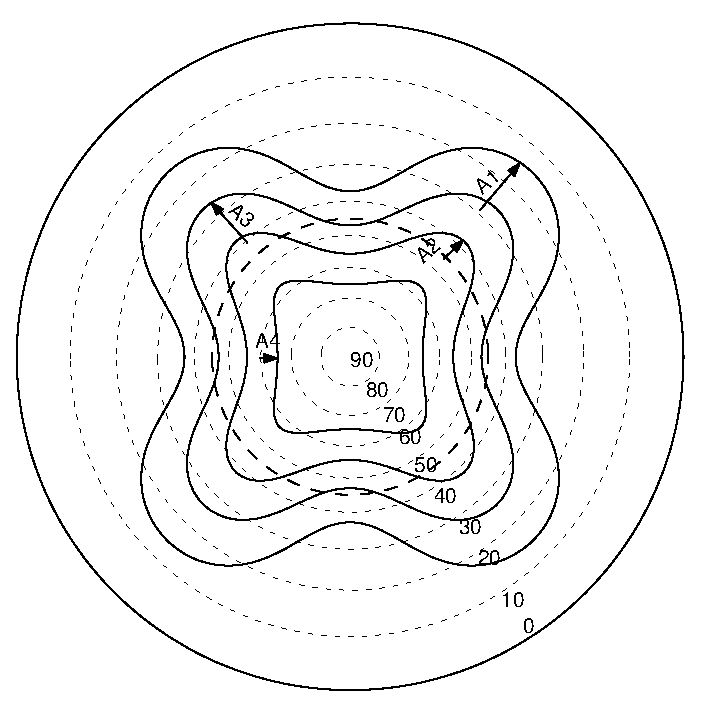
\includegraphics[scale=0.85]{IMAGES/ampmeas.eps}
	\caption{Various amplitude measurement methods}
	\label{fig:ampmeas}
\end{figure} To be consistent we require just one mean state but due to the multitude of wave shapes that are possible we see that there are an infinite number of mean states about which we can measure wave deviation. We must therefore decide on exactly where to measure amplitude from for any given wave. Because Rossby wave activity is predominantly associated with the mid-latitude regions and also because $\phi=\pm \pi/4$ represents the mid point between the equator and either pole, we choose the mean reference level as the latitude circle located 45 degrees from the equator in either hemisphere.

We now note that when we refer to progressive Rossby waves we actually mean a progressive-wave pattern as a perturbation from a base zonal flow state. As we have already shown in Section~\ref{sec:incompbase}, associated with the base zonal flow state is a zonal free-surface state which has level surfaces lying along latitude circles of constant $\phi$. For a given total system volume we can calculate the height of the zonal flow free-surface contours at $\phi=\pm \pi/4$ and then use these base levels to measure how the zonal flow state is deformed when a progressive Rossby wave structure is present. That is, we first record the base zonal height, denoted $h_{\text{bz}}$, of the free-surface at $\phi=\pm \pi/4$ when there is no Rossby wave structure, and then when a Rossby wave structure is present we find the height contour at the level $h_{\text{bz}}$ and measure exactly how this \index{Amplitude!measurement method}level surface has been modified from its base zonal state.

We also note that the amplitudes indicated in Figure~\ref{fig:ampmeas} will in general not be the same in both the equator-ward and pole-ward directions, with the divergence between the two growing as the overall wave amplitude grows. Because of the topology of the sphere it is possible for a Rossby wave to extend further towards the equator than towards the pole where the lines of longitude converge. Thus to record $\mathcal{A}$ effectively we will need to measure both the equator-ward and pole-ward deflections, which we denote \index{Amplitude!$\mathcal{A}_{\text{e}}$}$\mathcal{A}_{\text{e}}$ and \index{Amplitude!$\mathcal{A}_{\text{p}}$}$\mathcal{A}_{\text{p}}$ respectively. Associated with these separate but related amplitudes we define a simple averaged amplitude, the mean of the two values, to be
\begin{equation}
\mathcal{A}_{\text{ave}}=\frac{\mathcal{A}_{\text{e}}+\mathcal{A}_{\text{p}}}{2}.
\end{equation}
In \index{Amplitude!$\mathcal{A}_{\text{ave}}$}forthcoming sections when we present specific results we will plot the wavespeed $c$ versus each of the above defined amplitudes, namely $\mathcal{A}_{\text{e}}$, $\mathcal{A}_{\text{p}}$ and $\mathcal{A}_{\text{ave}}$.

\subsection{Parameters and Constants}
\label{subsec:incomparams}
Although this analysis is not specific to a given sphere size or mass it again seems reasonable, as in the linearized model, to use \index{parameter specification}parameters that closely approximate those of the Earth so that direct comparison can be made between existing meteorological models and observations. With this in mind we adopt the following values for the sphere specific parameters:
\begin{align}
a&=6.37122\times10^6\text{m},\\
\Omega&=\frac{2 \pi}{24\times3600}\approx7.272\times10^{-5}\,\text{s}^{-1},\\
g&=9.80616\,\text{m}\,\text{s}^{-2}.
\end{align}
Additionally we define each characteristic reference scale as
\begin{align}
v_{\mbox{\tiny ref}}&=40\,\text{m}\,\text{s}^{-1},\\
h_{\mbox{\tiny ref}}&=8.0\times10^{3}\text{m},\\
c_{\mbox{\tiny ref}}&=\frac{\Omega}{30}\approx2.4241\times10^{-6}\,\text{s}^{-1}.
\end{align}

For the dimensionless zonal flow parameter $\omega$ we will use two specific values. In the linearized model we were afforded the luxury of being able to specify a broad range of $\omega$ values with little overhead incurred in terms of time taken to numerically analyze the problem. Unfortunately, in the nonlinear model, we are no longer able to investigate the solution dependency on $\omega$ without incurring a significant increase in the computation time. This is because at each value of $\omega$ chosen we must compute a complete solution curve for the $c$ versus $\mathcal{A}$ relationship which involves many possible values of the wavespeed, rather than the single value computed in the linearized model. On average, to compute a complete solution curve for a fixed value of $\omega$, many weeks of computational time is required for programs executing on the previously documented hardware specifications in Section~\ref{subsec:compinfo}.

For this reason it was decided to restrict the investigation to two specific values of the parameter $\omega$. The first value is consistent with the angular speed $\omega$ used in the test set proposed by Williamson~et~al.~\cite{Williamson:STS}. The second value, chosen to be 80\% of the first value,  provides a slower and perhaps physically more realistic value for the super rotation rate. In dimensionless form the two values are given by
\begin{align*}
\omega_1 & \approx 1.25, \\
\omega_2 & \approx 1.0.
\end{align*}
The particular values above are obtained by noting that Williamson~et~al. use a dimensional value for $\omega$ of $7.848\times10^{-6}\,\text{s}^{-1}$, a value first introduced by Phillips\cite{Phillips:NIP}. In order to convert this to a dimensionless number it is necessary to multiply by the radius of the Earth and divide by the reference velocity scale so that
\begin{align*}
\omega_1 & =\frac{7.848\times10^{-6}a}{v_{\mbox{\tiny ref}}}\approx1.25, \\
\omega_2 & = 80\% \omega_1 \approx 1.0.
\end{align*}

It is also necessary to specify a base volume \index{$V_z$, zonal flow volume}$V_z$ for the system, to be used in the volume specification equation given by \eqref{eq:volcon}. For this study the value was chosen to be the total volume contained between the surface of the sphere and the free-surface shape defined by the zonal flow with parameters $h_o=1$ and $\omega=1.25$. Thus the base volume is simply the total volume of the atmosphere corresponding to purely zonal flow with parameters equivalent to those used in Williamson~et~al.\cite{Williamson:STS}.

\subsection[Results for $\kappa=4$, $\omega=1.25$]{Results for \boldmath$\kappa=4$, $\omega=1.25$}
\label{subsec:incomnlk4w125}
We now examine results obtained by solving the equations using the numerical methods previously outlined. Because the process of root finding is quite sensitive to the initial approximation to the root we use the first type of bootstrapping defined in Section~\ref{subsec:bootstrap} to find an initial small-amplitude solution based on the linearized result for equivalent parameter values in the model. Once we have obtained this small amplitude nonlinear solution we then slowly \index{forcing!amplitude}force the wave amplitude by holding coefficient $H_{1,1}$ fixed throughout the calculation and increasing its value between successive runs of the program. Using this technique we build up a picture of the overall relationship between the wavespeed and the amplitude.

Figure~\ref{fig:CvsAk4w125} shows the three solution curves when $\kappa=4$ and $\omega=1.25$ for each of the three measures of amplitude $\mathcal{A}_{\text{e}}$, $\mathcal{A}_{\text{p}}$ and $\mathcal{A}_{\text{ave}}$ defined previously in Section~\ref{subsec:ampmeas}. The truncation levels are $M=20$ and $N=20$ so that each series has a total of 400 coefficients, with a total of 1200 unknowns for the problem. Results were initially computed at a lower truncation level of $M=N=10$ to ascertain the general nature of the relationship. Once the nature of the solution was established the truncation was increased.

\begin{figure}[htbp]
\psfrag{Ap}{\small $\mathcal{A}_{\text{p}}$}
\psfrag{Ae}{\small $\mathcal{A}_{\text{e}}$}
\psfrag{Aave}{\small $\mathcal{A}_{\text{ave}}$}
\psfrag{Wavespeed}{\scriptsize Wavespeed, $c$}
\psfrag{Amplitude}{\scriptsize Amplitude (degrees)}
\psfrag{Linearised}{\scriptsize Linearized solution}
	\centering
		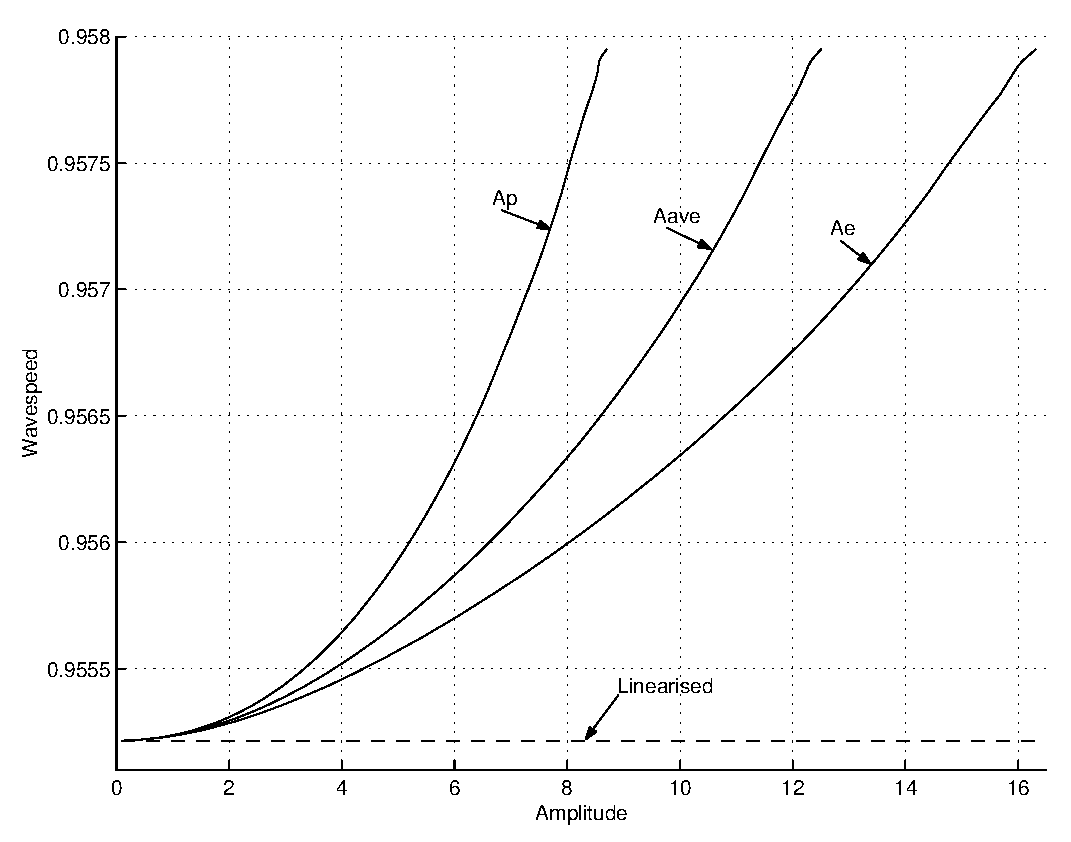
\includegraphics[scale=0.75]{IMAGES/CvsAk4w125.eps}
	\caption{Incompressible wavespeed versus amplitude for $\kappa=4$ and $\omega=1.25$}
	\label{fig:CvsAk4w125}
\end{figure}
The error tolerance on the $L^1$ norm of the residual vector was set at $10^{-12}$, leading to average individual residual errors of the order of $10^{-15}$ or less. The agreement between the two levels of representation was found to be excellent with results at the higher truncation level only differing marginally from those at the lower level, providing evidence for the numerical convergence of the solutions calculated. In particular, the third type of bootstrapping outlined in Section~\ref{subsec:bootstrap} was used to increase the truncation level beyond $M=N=20$ for a random sample of points on the solution curve, and in all cases these higher resolution solutions were found to differ negligibly from those for $M=N=20$, and, at least for small amplitude, from those of $M=N=10$ as well.

The linearized solution is included and indicated in Figure~\ref{fig:CvsAk4w125}, showing that for small amplitude waves the linear and nonlinear solutions are essentially equivalent. As the amplitude increases the wavespeed also increases, with the curve initially being tangential to the linearized result for small $\mathcal{A}$ but diverging from the linearized result and increasing more rapidly as $\mathcal{A}$ becomes larger. This behaviour is as expected by analogy with other nonlinear wave calculations for gravitationally influenced incompressible fluids, notably those of Stokes \cite{Stokes:TOW}, Schwartz \cite{Schwartz:CEA} and Cokelet \cite{Cokelet:SGW}. These results, along with contributions from other key researchers in the field, are summarised in the review article by Schwartz \& Fenton \cite{Schwartz:SNW}.
\begin{figure}[htbp]
	\centering
		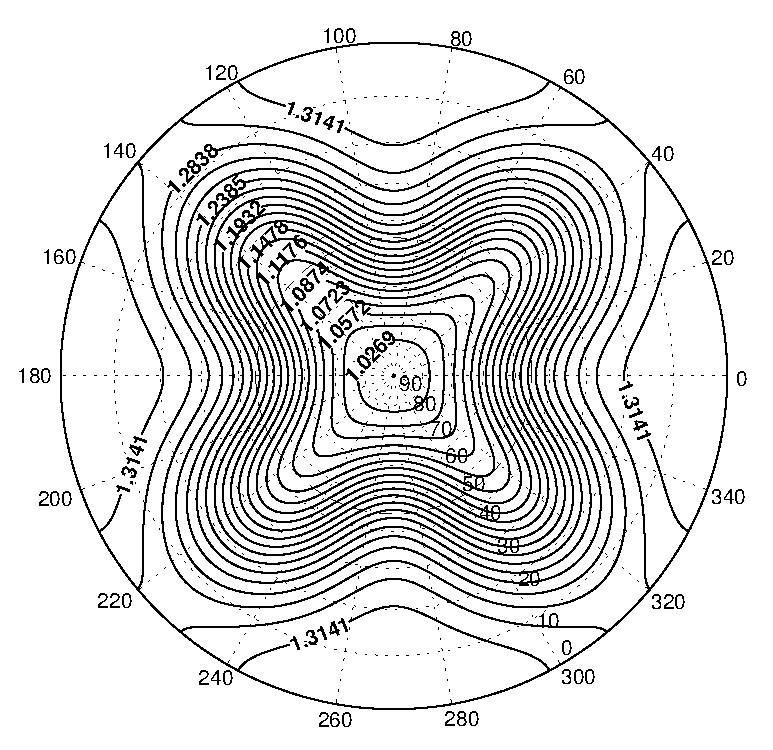
\includegraphics[scale=0.75]{IMAGES/k4w125fsend.eps}
	\caption{Incompressible shallow atmosphere free-surface contours for $\kappa=4$, $\omega=1.25$ at limit of computation. The average amplitude is $\mathcal{A}_{ave}=12.5104 (deg.)$ and the wavespeed is $c=0.9580$.}
	\label{fig:k4w125fsend}
\end{figure}

As the amplitude continues to increase the rate of wavespeed increase grows rapidly until, ultimately, a limiting case is achieved numerically, where a slight curling over of the curve is observed. The physical explanation of this limiting solution is not clear from this example computation. It is possible, for example, that a sharp crest might be formed somewhere in the flow field, as in the previously mentioned water-wave case studied by Stokes and later by Schwartz. Alternatively, it may be the case that the solution is topologically limited by enclosing bubbles, as found for the case of gravity waves with surface tension by Schwartz \& Vanden-Broeck~\cite{Schwartz:NSE}, and Chen \& Saffman~\cite{Chen:SGC}. However, an analysis of the free-surface contours at this limiting wavespeed and amplitude combination, as shown in Figure~\ref{fig:k4w125fsend}, suggests that no such behaviour is present. 

We suggest, however, that some type of \index{resonance!nonlinear}nonlinear resonance behaviour occurs, which is not accessible to this numerical scheme because of the complexity of the solution space and the  implied sensitivity of Newton's method to the initial guess used. Evidence supporting this statement is presented in the next section. Indeed, it is suspected that the limiting wavespeed-amplitude combination indicated in Figure~\ref{fig:CvsAk4w125} is only really limited by the numerical solution method and that, in reality, significantly faster and larger waves exist beyond the shown limit. Exhaustive attempts to find such larger waves were made using numerous methods. In particular the algorithm was changed so that the wavespeed became the \index{forcing!wavespeed}forcing parameter in an attempt to look for faster progressive waves; however convergence of the residual vector was not obtained. In addition, the results obtained with the lower truncation level of $M=N=10$ were found to converge for slightly larger amplitudes and wavespeeds, although it was then found that subsequent bootstrapping of these lower resolution solutions to ones at a higher resolution produced non-convergent residuals. We must therefore reject these results at this point until further analytical and numerical work can be done to investigate this behaviour.

\subsection[Results for $\kappa=4$, $\omega=1.0$]{Results for \boldmath$\kappa=4$, $\omega=1.0$}
\label{subsec:incomnlk4w1}
The solution curves shown in Figure~\ref{fig:CvsAk4w1} represent results obtained with the values $\kappa=4$ and $\omega=1.0$. The truncation levels were set at $M=N=15$ with initial curves mapped out using $M=N=10$; little overall difference was observed between the two resolutions. The error tolerance on the $L^1$ norm of the residual vector was set at $10^{-12}$, leading to average individual residual errors of the order of $10^{-15}$ or less. Like the previous example, the solution agrees well with the linearized result for small amplitude waves and as $\mathcal{A}$ increases so does the wavespeed $c$. However, as opposed to the previous case for $\omega=1.25$, distinct \index{resonance!branch}discontinuous jumps are now evident, dividing the solution curves into separate branches, between which no numerical solutions were able to be computed to adequate convergence. The individual branches have been labelled in the figure and will be refered to subsequently as branches 1 through 5 respectively.

\index{resonance!discrete branching}Discrete branching of the solution, as evidenced in the present results, is characteristic of nonlinear resonance interaction in general, in which certain energy states of the system can be viewed as sympathetically exciting the underlying wave motion, undergoing energy exchange between waves of different wavelengths in the process. Nonlinear resonance has been known to exist in complex nonlinear wave propagation problems for some time now. In the context of gravity waves with surface tension Wilton~\cite{Wilton:OR} encountered key values of the capillary number at which resonance occured. Schwartz \& Vanden-Broeck~\cite{Schwartz:NSE}, and Hogan~\cite{Hogan:SES1,Hogan:SES2,Hogan:SES3}, confirmed this behaviour in detail, by numerically solving the exact equations, and found that multiple simultaneous solution branches were possible. Forbes~\cite{Forbes:SWL1,Forbes:SWL2} also found resonant behaviour for surface waves of large amplitude beneath an elastic sheet. 
\begin{figure}[tbp]
\psfrag{Ap}{\small $\mathcal{A}_{\text{p}}$}
\psfrag{Ae}{\small $\mathcal{A}_{\text{e}}$}
\psfrag{Aave}{\small $\mathcal{A}_{\text{ave}}$}
\psfrag{Wavespeed}{\scriptsize Wavespeed, $c$}
\psfrag{Amplitude}{\scriptsize Amplitude (degrees)}
\psfrag{Linearised}{\scriptsize Linearized solution}
\psfrag{B1}{\scriptsize Branch 1}
\psfrag{B2}{\scriptsize Branch 2}
\psfrag{B3}{\scriptsize Branch 3}
\psfrag{B4}{\scriptsize Branch 4}
\psfrag{B5}{\scriptsize Branch 5}
	\centering
		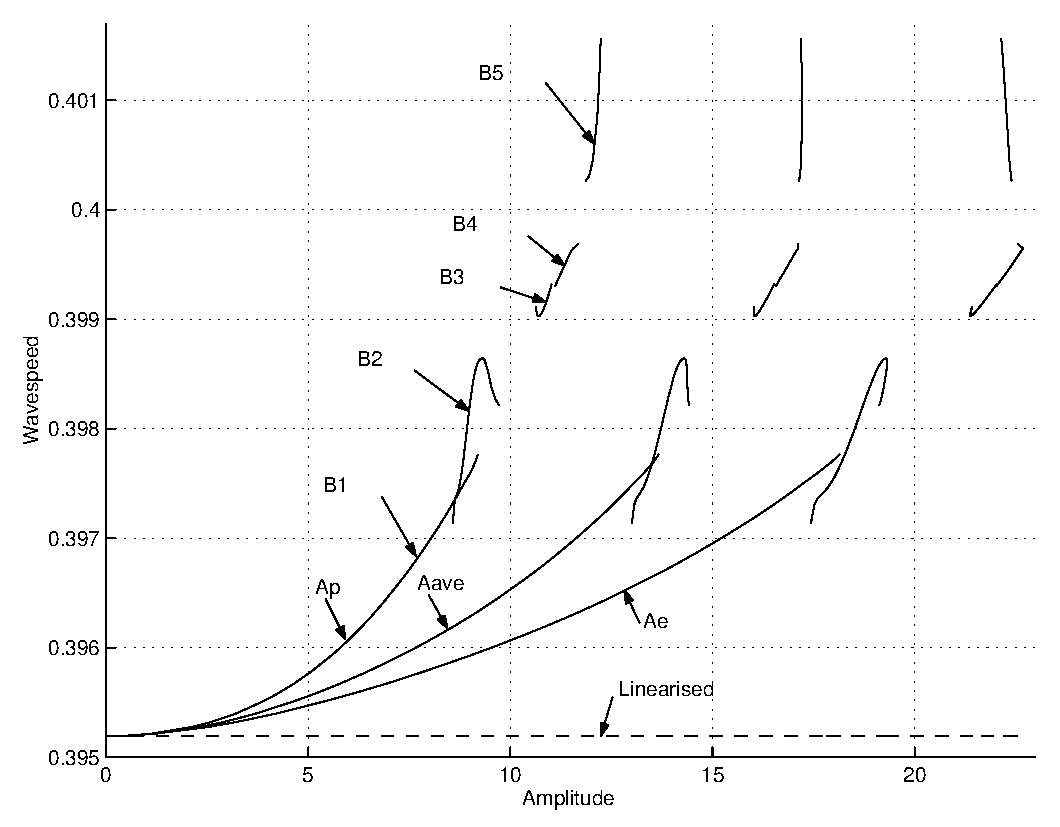
\includegraphics[scale=0.75]{IMAGES/CvsAk4w1.eps}
	\caption{Incompressible wavespeed versus amplitude for $\kappa=4$ and $\omega=1.0$}
	\label{fig:CvsAk4w1}
\end{figure}

In the meteorological context, nonlinear resonance behaviour has been studied by Longuet-Higgins \& Gill~\cite{Longuet:RIP} who showed that resonant interactions over time can exist between three waves, termed a resonant triad, obeying certain algebraic relationships relating the individual wavenumbers, associated with each physical dimension, and corresponding wavespeeds; their results are concerned with \index{resonance!planetary wave}planetary waves both on the $\beta$-plane and more generally on a spherical surface. Both Hoskins~\cite{Hoskins:SRH} and Baines~\cite{Baines:SPW} extend this work by considering the \index{stability!planetary wave}stability of planetary waves and calculating amplitudes required for instability based on triad interactions for specific types of Rossby-Haurwitz waves.

To understand how the resonance is occuring in this particular example we can view the system as being forced by the parametrized amplitude through the Fourier coefficient $H_{1,1}$. As $H_{1,1}$ increases we see $\mathcal{A}$ and $c$ also increasing until suddenly some of the Fourier modes in our series expansions are naturally excited  by the forcing and can absorb energy via nonlinear interactions. At this point resonance occurs and the system becomes unstable in the sense that unchanging progressive waves are no longer possible. We can thus think of resonance in this instance as a \index{resonance!parameter region}parameter region of, possibly highly oscillatory, transition between two stable progressive states for the full nonlinear time dependent problem. The fundamental nature of any resonance demands that the amplitude of the dominant harmonic wave grow in time. As we are only concerned with progressive waves this type of behaviour is excluded at the outset when we defined our travelling coordinate transform. However, as indicated by our results, the method used is still able to expose fundamental resonances of the system where full time dependence would be necessary to discern the complete behaviour of the dynamical system.
\begin{figure}[htbp]
	\centering
		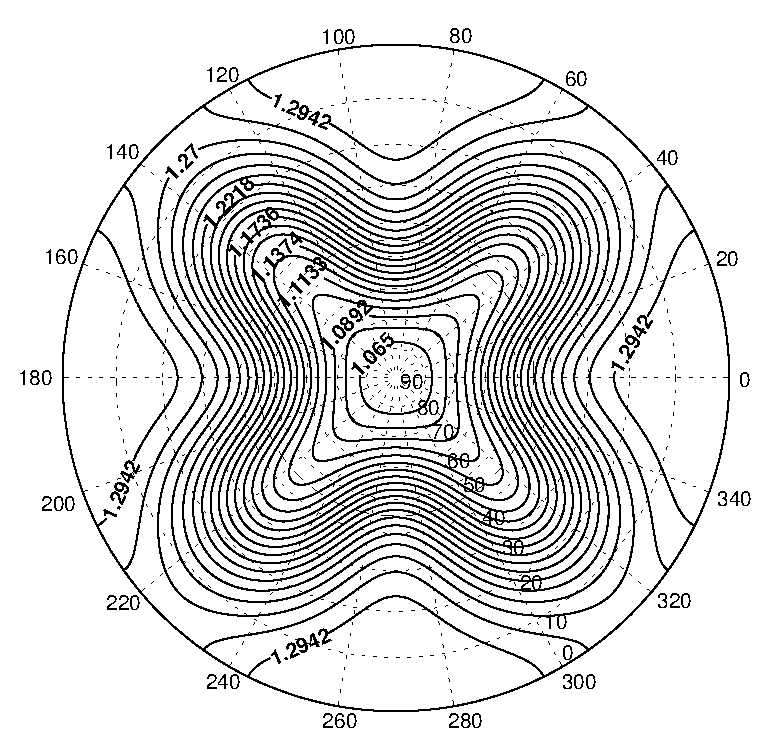
\includegraphics[scale=0.75]{IMAGES/k4w1fsb1end.eps}
	\caption{Incompressible shallow atmosphere free-surface contours at end of branch 1 for $\kappa=4$, $\omega=1.0$. The average amplitude is $\mathcal{A}_{ave}=13.6732 (deg.)$ and the wavespeed is $c=0.3978$.}
	\label{fig:k4w1fsb1end}
\end{figure}

The separate branches of the solution curve shown in Figure~\ref{fig:CvsAk4w1} can be classified, at least partially, in terms of the general associated height field structure and corresponding velocity vector field along each solution curve segment. On branch 1 we conclude that at no point in the flow does the fluid move counter to the general direction of the overall wave propagation direction and additionally that the only \index{stagnation point}stagnation points in the flow field are located at either of the two topological poles, as expected. The free-surface contours at the limiting upper value of branch 1 are shown in Figure~\ref{fig:k4w1fsb1end}. It is observed that the general character of these contours is quite similar to those obtained with both the linearized model and Rossby--Haurwitz theory of Section~\ref{subsec:rhandlincomp} of the previous chapter.

Not much difference was observed between the solutions along branch 1 and those along branch 2, with the general flow properties of the previous paragraph applying equally well here. It is also important to emphasize that the apparent intersection of branches 1 and 2 in the diagram is not a \index{bifurcation point}bifurcation point. Examination of the Fourier coefficients in the neighbourhood of the overlap shows distinctly different solution structure for each branch which fail to converge to a common set, despite the fact that the values of $\mathcal{A}$ and $c$ for the two branches coincide at this point. It would be possible to prove this with a simple analysis of the determinant of the Jacobian near the point of apparent intersection, as in Chen \& Saffman~\cite{Chen:SGC}; however the ease with which the Newton method iterates through this region seems to suggest that no further investigation is necessary with regard to the possible existence of a bifurcation. Additionally, the solution curve for the equatorial amplitude $\mathcal{A}_{\text{e}}$ does not contain the intersection, which confirms the presence of a resonance branch, instead of a simple bifurcation.

Solutions on branches 3 and above reveal richer dynamics in terms of more stagnation points in the flow field, \index{reverse flow}reverse flow leading to \index{localised circulation}localised circulation, and highly nonlinear wave profiles. The main difference between the lower solution branches 1 and 2 and the upper solution branches 3, 4 and 5 can be expressed by examining the number of \index{stagnation point}stagnation points in the flow field, disregarding the obvious polar stagnation points that all solutions must have by definition of the series expansions themselves. It is evident that for solutions on branches 3 and higher, all have stagnation points located \index{stagnation point!symmetrical location}symmetrically on the equator about the coordinate lines $\eta=\frac{2n\pi}{\kappa}$, for $n=0,1,\ldots,\kappa-1$. The exact position of these stagnation points was noted to change as the amplitude varied, although typically they were located quite close to the symmetry lines themselves. In between the two stagnation points the fluid was observed to flow counter to the general direction of the progressive-wave movement. The height field was examined for small-scale localised high pressure cells at these points of circulation, but none were found. However this does not contradict geostrophic theory, which is primarily valid at mid latitudes rather than at the equator.

\begin{figure}[htbp]
	\centering
		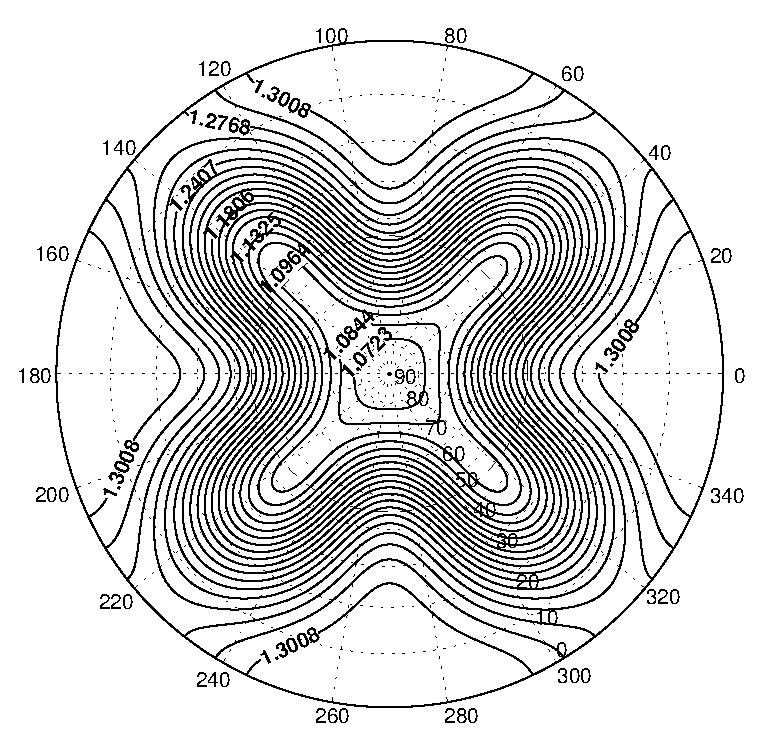
\includegraphics[scale=0.75]{IMAGES/k4w1fsb4end.eps}
	\caption{Incompressible shallow atmosphere free-surface contours at end of branch 4 for $\kappa=4$, $\omega=1.0$. The average amplitude is $\mathcal{A}_{ave}=17.11662 (deg.)$ and the wavespeed is $c=0.3997$.}
	\label{fig:k4w1fsb4end}
\end{figure}

Figure~\ref{fig:k4w1fsb4end} shows a typical free-surface contour plot for solutions along branches 3 and 4. The figure actually shows the contours at the limiting upper value of branch 4 and so represents the maximum allowable amplitude for waves on branch 4. It seems, from an analysis of the velocity fields and height contours, that the qualitative difference between waves on branches 3 and 4 is negligible. Nonetheless, a distinct gap was encountered when trying to establish the continuity of the solution between branches 3 and 4. Further investigation is needed to establish the key qualitative differences between these two branches, although this is both beyond the scope and computational capability of the present work.

Of particular note is the way in which low-level polar heights, and hence pressures, are seen to move equator-ward for solutions along these branches. It is suspected that the limiting factor for wavespeeds and amplitudes towards the upper end of branch 4 is directly related to the topology of the low-level free-surface contours which are not able to bend inwards any further without creating an isolated cut-off low pressure system in the flow field. This statement is supported by the following analysis of branch 5 solutions.

\begin{figure}[htbp]
	\centering
		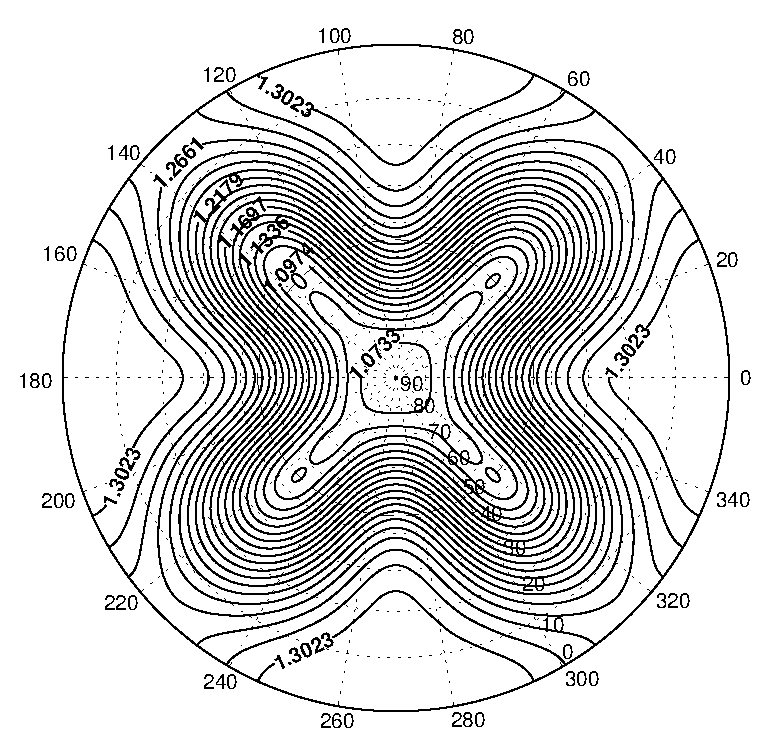
\includegraphics[scale=0.75]{IMAGES/k4w1fsb5end.eps}
	\caption{Incompressible shallow atmosphere free-surface contours at end of branch 5 for $\kappa=4$, $\omega=1.0$. The average amplitude is $\mathcal{A}_{ave}=17.11662 (deg.)$ and the wavespeed is $c=0.4016$.}
	\label{fig:k4w1fsb5end}
\end{figure}
The highly nonlinear free-surface height contours for the upper end of branch 5 are shown in Figure~\ref{fig:k4w1fsb5end}. It is immediately evident that solutions along this branch have the distinguishing feature of \index{pressure!cut-off low}cut-off low pressure cells which are isolated from the general progressive-wave structure. In addition to the already mentioned stagnation points in the flow field for waves on branches 3 and higher, more stagnation points are introduced for waves on the fifth branch, this time occuring close to the poles of the coordinate system rather than near the equator. It was initially suspected that the centre of each cut-off low pressure cell must be a stagnation point; however careful analysis of the velocity vector field did not confirm this. Nonetheless the velocity in the vicinity of these cells is quite small compared to the rest of the flow field and can almost be described as circulatory about the centre of each cell.

It is of interest to note that the stagnation points introduced for branch 5 solutions occur immediately below each cut-off low pressure cell as indicated in figure~\ref{fig:k4w1fsvvb5end}. Also shown are all previously mentioned stagnation points as well as regions of circulation, labeled reverse flow. We can conclude that generally the flow is seen to be geostrophic in the sense that the streamlines are nearly parallel to the isobars. This is clearly true in the neighbourhood of the perturbed $\phi=\pm\pi/4$ zonal flow contour that forms the basis of the numerical analysis in this section.
\begin{figure}[htbp]
\psfrag{Stagnation points}{\scriptsize Stagnation points}
\psfrag{Reverse Flow}{\scriptsize Reverse flow}
	\centering
		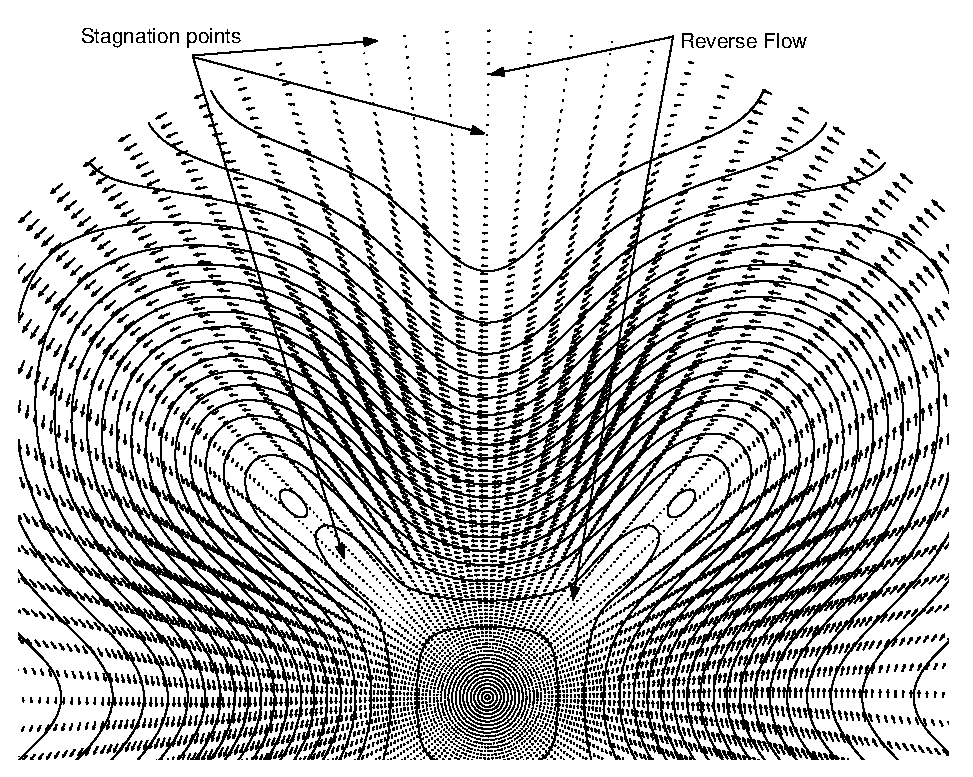
\includegraphics[scale=0.75]{IMAGES/k4w1fsvvb5end.eps}
	\caption{Incompressible shallow atmosphere free-surface contours with corresponding velocity vector field at end of branch 5 for $\kappa=4$, $\omega=1.0$. The average amplitude is $\mathcal{A}_{ave}=17.11662 (deg.)$ and the wavespeed is $c=0.4016$.}
	\label{fig:k4w1fsvvb5end}
\end{figure}

The fate of the solution curves past the end of branch 5 is still uncertain. Attempts were made to compute more points beyond the limits shown but in all cases convergence was not achieved. It might be that our numerical method is not well suited to computing past points where the slope of the curve is nearly infinite, in which case improved techniques are required to investigate the behaviour past the limit shown. Alternatively this may be close to the \index{Amplitude!maximum allowable}maximum allowable amplitude of the system, imposed as a consequence of the finite size and topology of the sphere. An analysis of the constraints of potential vorticity conservation of Rossby waves on a $\beta$-plane by Lindzen \& Schoeberl~\cite{Lindzen:NLR} revealed that there are finite limits to the size of Rossby wave amplitudes. This reasoning should apply even more so to the sphere where the finite size becomes an important attribute of the problem.

\subsection[Results for $\kappa=5$, $\omega=1.25$]{Results for \boldmath$\kappa=5$, $\omega=1.25$}
\label{subsec:incomnlk5w125}
\begin{figure}[htbp]
\psfrag{Ap}{\small $\mathcal{A}_{\text{p}}$}
\psfrag{Ae}{\small $\mathcal{A}_{\text{e}}$}
\psfrag{Aave}{\small $\mathcal{A}_{\text{ave}}$}
\psfrag{Wavespeed}{\scriptsize Wavespeed, $c$}
\psfrag{Amplitude}{\scriptsize Amplitude (degrees)}
\psfrag{Linearised}{\scriptsize Linearized solution}
\psfrag{B1}{\scriptsize Branch 1}
\psfrag{B2}{\scriptsize Branch 2}
	\centering
		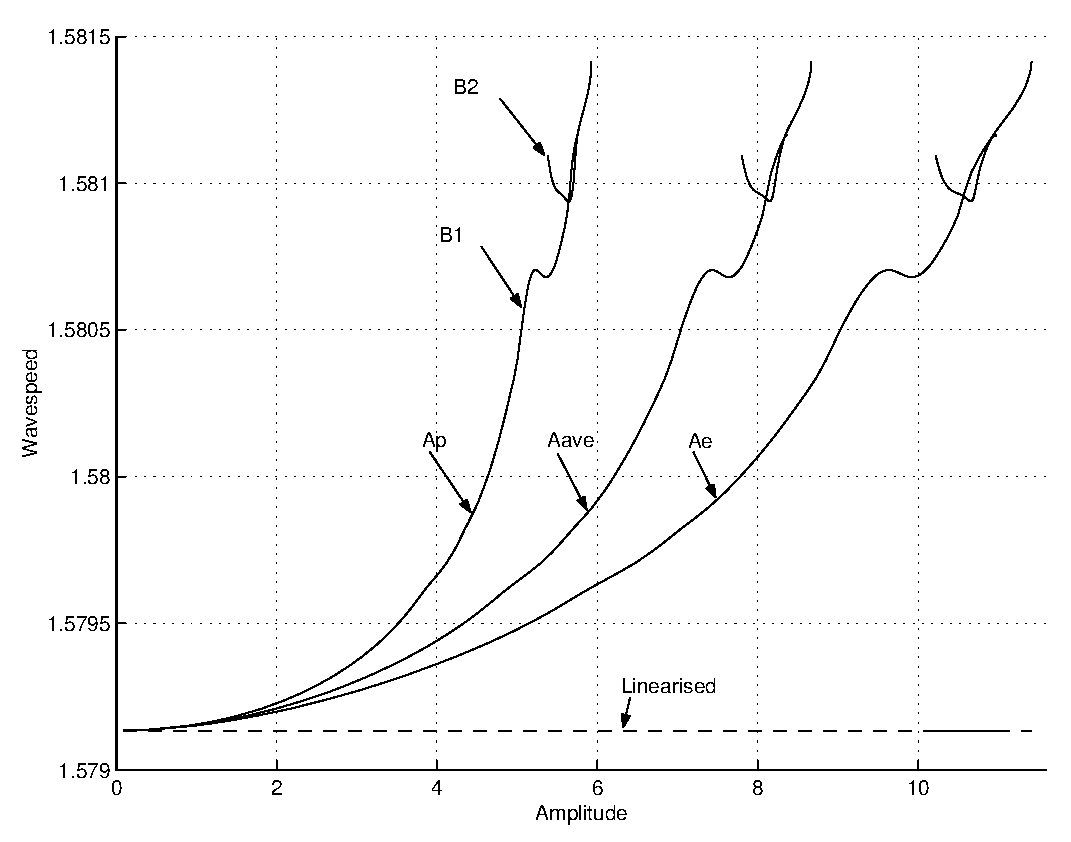
\includegraphics[scale=0.75]{IMAGES/CvsAk5w125.eps}
	\caption{Incompressible wavespeed versus amplitude for $\kappa=5$ and $\omega=1.25$}
	\label{fig:CvsAk5w125}
\end{figure}

It is of interest to study how the dynamical system behaves with an alternative value of the wave number $\kappa$. We now present results obtained with $\kappa=5$, using the same pair of values ($\omega=1.25$ and $\omega=1.0$) for the dimensionless zonal flow super rotation; in this section we examine the case $\omega=1.25$. Figure~\ref{fig:CvsAk5w125} shows the computed wavespeed versus amplitude relationship using a truncation of $M=N=20$. The error tolerance on the $L^1$ norm of the residual vector was set at $10^{-12}$, leading to average individual residual errors of the order of $10^{-15}$ or less.

The same general trend as for $\kappa=4$ is encountered here for $\kappa=5$, with the linearized solution being a good approximation to the nonlinear solution for small $\mathcal{A}$ and the wavespeed becoming increasingly greater as the amplitude is increased. It appears that the use of $\kappa=5$ introduces a new phenomenon in the form of a localised cubic structure located near $c\approx1.5807$. It was initially suspected that this was in fact two distinct branches separated by a resonance; however it was possible to compute continuously through this region, using a very small step size, without encountering any non convergent solutions. 

Therefore it seems that there are at least two explanations for this behaviour. The first is that there is in fact a resonance occuring near the point of inflexion, but existing on such a small scale that we were unable to detect it on any occasion. This does not seem very likely given the nature of the previous nonlinear resonances observed for the case $\kappa=4$, $\omega=1.0$. The second explanation is that this is a feature of the dynamics and forcing, in which energy exchange between certain wavelengths is taking place in such a maner as to increase the overall amplitude while at the same time reducing the wavespeed. If so, this would represent a type of \index{resonance!damped}damped resonance, but careful analytical work, beyond the scope of this study, would be needed to identify the physical nature of the damping mechanism. Despite this localised reversal of the general trend of the graph, no obvious distinguishing features are visible when we examine the free-surface contours and velocity vector field in the vicinity of this solution region. This fact seems to support the conjecture that separate resonance branches do not exist in this case.

Two separate solution branches were found to exist towards the upper end of the curve when the limiting amplitude-wavespeed combination was approached. Because it is not entirely clear from the figure, it needs to be emphasized that the first branch terminates in the vicinity of $c\approx1.5812$; thus the highest possible wavespeed indicated is at the right end of branch 2. It is again unlikely that the apparent intersection of the two branches is a sign of a simple \index{bifurcation}bifurcation, for reasons outlined in the previous section.

For the left end of the second branch, numerical results have in fact been computed well beyond the termination point shown in the figure. However, it appears that they are of questionable validity due to increasing numerical error along that branch and have therefore not been shown. The ultimate fate of this upper branch is not clear and may perhaps require alternative numerical techniques to reveal. In any event it is possible that this branch is physically unstable, the system preferring the lower wavespeed over the higher one, and so would generally not be observed in practice. It is even possible that a physical instability in this branch might produce a numerical instability, since the numerical iteration process may be equivalent to stepping forward in time, as has been shown in various applications of the Peaceman-Rachford ADI method to the heat equation, documented in Ames~\cite[page 149]{Ames:NMP}.

\begin{figure}[htbp]
	\centering
		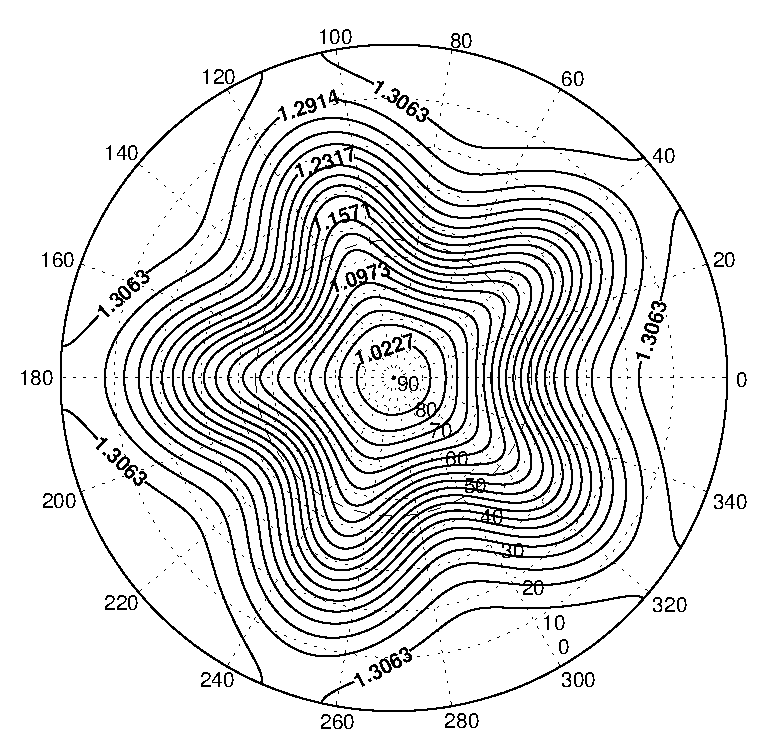
\includegraphics[scale=0.75]{IMAGES/k5w125fsb1end.eps}
	\caption{Incompressible shallow atmosphere free-surface contours at end of branch 1 for $\kappa=5$, $\omega=1.25$. The average amplitude is $\mathcal{A}_{ave}=8.3678 (deg.)$ and the wavespeed is $c=1.5812$.}
	\label{fig:k5w125fsb1end}
\end{figure}

Typical free-surface contours of the system are presented in Figure~\ref{fig:k5w125fsb1end}, showing the nature of the solution at the end of branch 1. In contrast to the highly nonlinear structures computed at the end of the curve for $\kappa=4$ and $\omega=1.0$, these contours exemplify the significantly smaller maximum amplitude for which a convergent wavespeed was able to be calculated. In addition, no defining qualitative features of the velocity field were found that could be used to distinguish easily between the two solution branches. It is possible that more solution curves exist beyond those that are indicated; however attempts to find such solutions were not successful. 

\subsection[Results for $\kappa=5$, $\omega=1.0$]{Results for \boldmath$\kappa=5$, $\omega=1.0$}
\label{subsec:incomnlk5w1}
For completeness we present results in this final section for $\kappa=5$ and $\omega=1.0$. Figure~\ref{fig:CvsAk5w1} shows the computed solution curves obtained with the truncation level $M=N=15$. The error tolerance on the $L^1$ norm of the residual vector was again set at $10^{-12}$. The general features of this figure are less remarkable than those for the preceding set of results obtained with $\omega=1.25$, although there is some evidence for a similar localised cubic structure, this time in the vicinity of $c=0.99395$. The severity of this local cubic behaviour, however, is significantly less noticeable and does not substantially influence the general increase of $c$ with $\mathcal{A}$. As in all previous solution curves presented, the results here agree well with the linearized value of the wavespeed for small values of the amplitude.
\begin{figure}[htbp]
\psfrag{Ap}{\small $\mathcal{A}_{\text{p}}$}
\psfrag{Ae}{\small $\mathcal{A}_{\text{e}}$}
\psfrag{Aave}{\small $\mathcal{A}_{\text{ave}}$}
\psfrag{Wavespeed}{\scriptsize Wavespeed, $c$}
\psfrag{Amplitude}{\scriptsize Amplitude (degrees)}
\psfrag{Linearised}{\scriptsize Linearized solution}
	\centering
		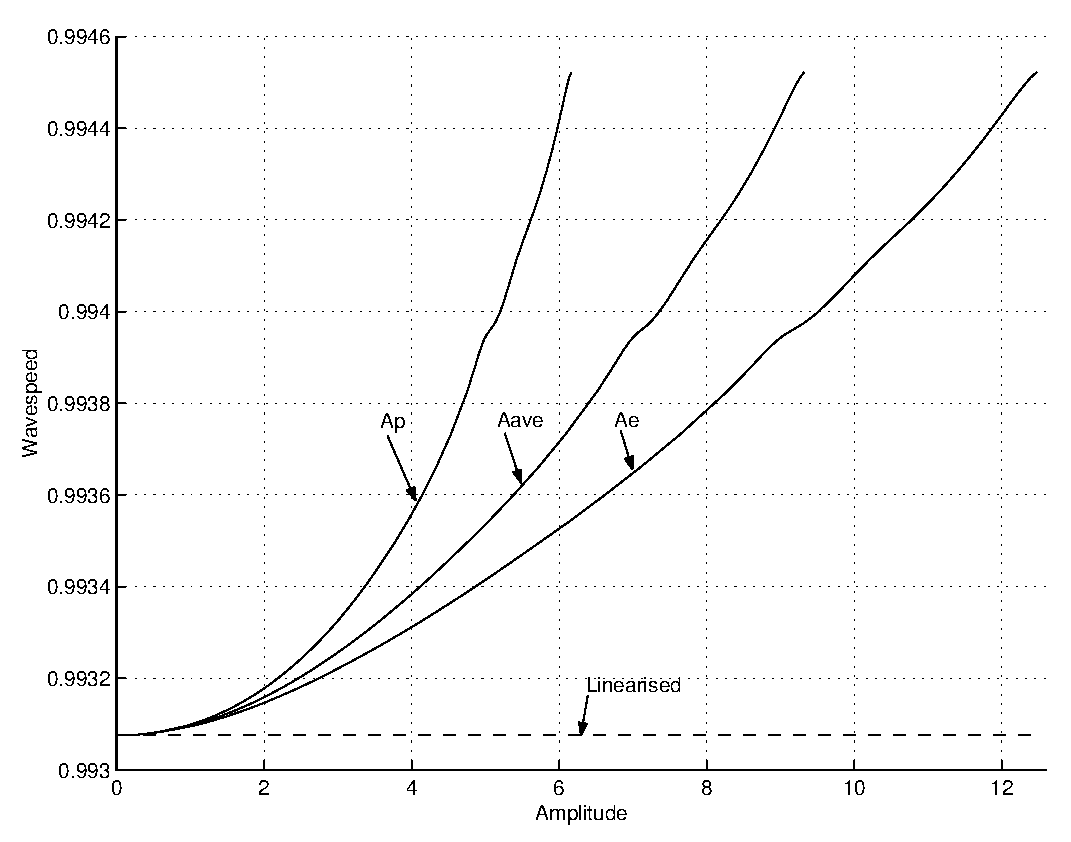
\includegraphics[scale=0.75]{IMAGES/CvsAk5w1.eps}
	\caption{Incompressible wavespeed versus amplitude for $\kappa=5$ and $\omega=1.0$}
	\label{fig:CvsAk5w1}
\end{figure}

Typical free-surface contours at the right end of the one and only computed branch are shown in Figure~\ref{fig:k5w1fsend}. The waves shown are in general highly nonlinear and it should be noted that the maximum possible amplitude obtained with this slower zonal super rotation speed is larger than that obtained with $\omega=1.25$. No additional stagnation points in the flow field were observed, as in the previous case, and consequently all fluid flow was found to be in the same direction as the direction of propagation of the progressive-wave. 

\begin{figure}[htbp]
	\centering
		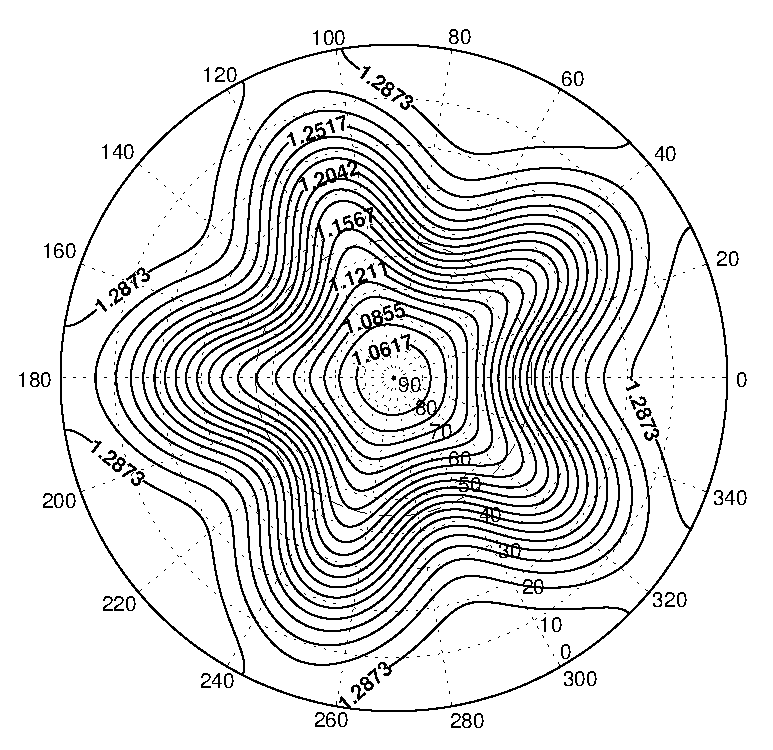
\includegraphics[scale=0.75]{IMAGES/k5w1fsend.eps}
	\caption{Incompressible shallow atmosphere free-surface contours at end of branch 1 for $\kappa=5$, $\omega=1.0$. The average amplitude is $\mathcal{A}_{ave}=9.3175 (deg.)$ and the wavespeed is $c=0.9945$.}
	\label{fig:k5w1fsend}
\end{figure}

It is again suspected that there are in fact more solution branches in addition to the one shown in Figure~\ref{fig:CvsAk5w1}. To support this statement we argue that the general nature of the flow field at the limiting computed value seems to be rather well behaved with no clearly identifiable limiting topological features. Unsuccessful attempts were made to bootstrap the limiting solutions to those on another higher branch; in all cases adequate convergence of the residual vector was not achieved. 

It is also of interest to point out that the general computed values of the wavespeed for this set of results are similar in magnitude to those computed for $\kappa=4$ and $\omega=1.25$. In so far as the qualitative nature of both solution curves is the same, it seems reasonable to speculate that all solutions in the vicinity of this wavespeed behave in a similar manner. That is to say that a general increase of $c$ is seen with increasing $\mathcal{A}$ for all values of $\kappa$ and appropriate value of $\omega$.

\section{Closing Remarks}
In this chapter we have successfully solved the complete nonlinear equations governing shallow atmosphere free-surface flow with embeded progressive Rossby wave structures. Solutions in the form of finite Fourier series were obtained using a collocation method with an associated Newton iterative scheme. By starting close to the linearized solutions computed in the previous chapter and forcing the amplitude to increasingly larger values we were able to successfully step along the wavespeed versus amplitude solution curves for specific values of the parameters $\kappa$ and $\omega$.

Results obtained show that a relationship exists between increasing wave amplitude and wavespeed; these are similar to the well know results for gravity influenced free-surface waves. For the specific case of $\kappa=4$ and $\omega=1.0$ we found substantial evidence for nonlinear resonance in the system, with adjacent solution branches being separated by areas in which no solutions could be computed to within reasonable convergence. At the limit of computability it was shown that highly nonlinear wave profiles are possible with areas of cut off low pressure being a key feature of the system at this critical limit. It is suspected that this behaviour exists in general, at least to some extent, for all solutions that were investigated; however attempts to confirm this have thus far been unsuccessful with questionable results. It is highly unlikely that numerical methods alone can answer this existence question. Analytical techniques may be required to address this issue, however these are beyond the scope of the present investigation.
